\section{Experiments}\label{sec:experiments}

\begin{itemize}
    \item \lau{Put pas tense everywhere.}
    \item \todo{Update throughout (also in figures): $E \rightarrow E_\text{OR}, OR \rightarrow L_\text{OR}$, and use $L_\text{DE}$.}
    \item \mdeff{In general, we should try to make the text in figures larger. A trick I use in matplotlib is to lower the figure size, e.g., \texttt{fig = plt.figure(figsize=(4, 4))}}.
    \item \mdeff{We now have one figure per section. That's good, it makes the story of each section easy to grasp.}
\end{itemize}

To evaluate our method, we started with the orientation recovery experiments that included tests of feasibility and sensitivity to distance estimation error.
We then learned the distance using a SiameseNN and compared its performance with the baseline.
%After developing and tuning the architecture of the network for the distance estimation, we continue by introducing the perturbation to the projections.  and the network architecture is adjusted
The robustness of the network to perturbations is then evaluated.
Finally, we ran the whole machine learning pipeline to recover the orientations from estimated distances.

\subsection{Experimental conditions}\label{sec:results:data}

\paragraph{Proteins.}
We considered two proteins (\figref{pdb-proteins}): the $\beta$-galactosidase, a protein with a dihedral (D2) symmetry, and the lambda excision HJ intermediate (HJI), an asymmetric protein with local cyclic (C1) symmetry.
Their deposited PDB atomic models are \texttt{5a1a}~\cite{bartesaghi2015betagal} and \texttt{5j0n}~\cite{laxmikanthan2016structure}, respectively.
For each atomic model, we generated the ground truth by fitting a 5\AA\ density map in Chimera~\cite{pettersen2004ucsf}, which gave us a volume of $110 \times 155 \times 199$ voxels for the $\beta$-galactosidase, and a volume of $69 \times 57 \times 75$ voxels for the HJI.

\mdeff{How should we refer to the proteins beyond this point? Symmetric vs asymmetric, $\beta$-galactosidase vs HJI, or \texttt{5a1a} vs \texttt{5j0n}. It should be consistent. I'd vote for \texttt{5a1a} vs \texttt{5j0n}, and refer to the asymmetry if relevant for the experiment, explaining why.}

\begin{figure}[ht!]
    \centering
    \begin{minipage}[b]{0.55\linewidth}
        \centering
        \begin{subfigure}[b]{0.49\linewidth}
            \centering
            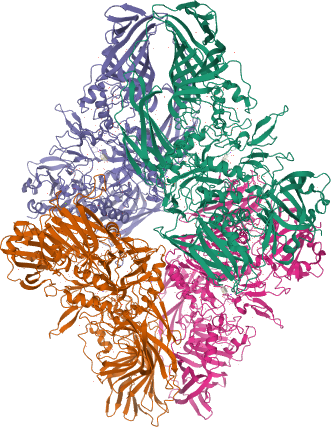
\includegraphics[height=5cm]{figures/5a1a_pdb.png}
            \caption*{\texttt{5a1a}}
        \end{subfigure}
        \hfill
        \begin{subfigure}[b]{0.42\linewidth}
            \centering
            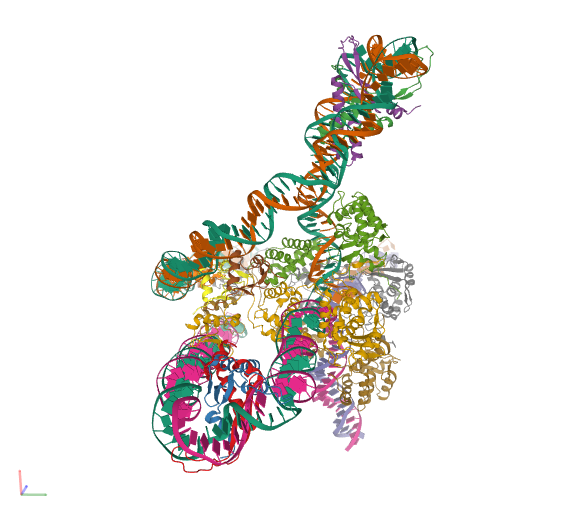
\includegraphics[height=5cm]{figures/5j0n_pdb.png}
            \caption*{\texttt{5j0n}}
        \end{subfigure}
        \caption{%
            Ground-truth proteins: the $\beta$-galactosidase (\texttt{5a1a})~\cite{5a1a_pdb}, and the lambda excision HJ intermediate (\texttt{5j0n})~\cite{5j0n_pdb}.
        }\label{fig:pdb-proteins}
    \end{minipage}
    \hfill
    \begin{minipage}[b]{0.35\linewidth}
        \centering
        \begin{subfigure}[b]{0.49\linewidth}
            \centering
            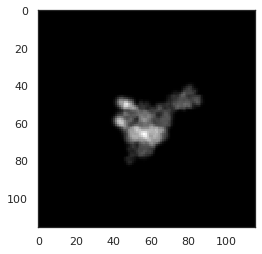
\includegraphics[width=0.8\linewidth]{figures/5j0n_noise0}
            \caption*{$\mathbf{P}_{\bth} \mathbf{x}$}
        \end{subfigure}
        \hfill
        \begin{subfigure}[b]{0.49\linewidth}
            \centering
            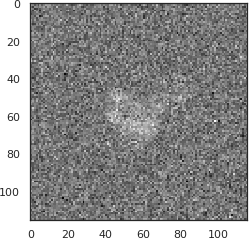
\includegraphics[width=0.8\linewidth]{figures/5j0n_noise16}
            \caption*{$\mathbf{P}_{\bth} \mathbf{x} + \mathbf{n}$}
    %, \; \mathbf{n} \sim \mathcal{N}(0, 16\mathbf{I})$}
        \end{subfigure}
        \\ \vspace{1em}
        \begin{subfigure}[b]{0.49\linewidth}
            \centering
            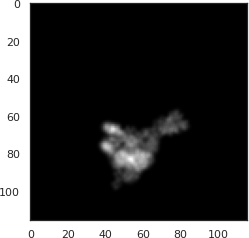
\includegraphics[width=0.8\linewidth]{figures/5j0n_translated}
            \caption*{$\mathbf{S}_{\mathbf{t}} \mathbf{P}_{\bth} \mathbf{x}$}
        \end{subfigure}
        \hfill
        \begin{subfigure}[b]{0.49\linewidth}
            \centering
            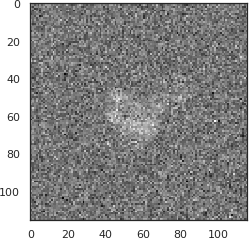
\includegraphics[width=0.8\linewidth]{figures/5j0n_noise16_translated}
            \caption*{$\mathbf{S}_{\mathbf{t}} \mathbf{P}_{\bth} \mathbf{x} + \mathbf{n}$}
        \end{subfigure}
        \caption{%
            Example projections of \texttt{5j0n}.
            % (a)~unperturbed, (b)~noisy, (c)~shifted, (d)~noisy and shifted.
        }\label{fig:different-projections}
    \end{minipage}
\end{figure}

\paragraph{Projections.}
From these ground truths, we generated $5,000$ synthetic projections of size $275\times 275$ and $116\times 116$, respectively, using the ASTRA projector~\cite{van2015astra}.
Our projection generator supports two orientation samplings: (i) sampling the Euler angles $\bth=(\theta_3,\theta_2,\theta_1)$ 
%\mdeff{Consistency: we used $\bth=(\theta_3,\theta_2,\theta_1)$ before. Which is better? Motivation for $(\theta_3,\theta_2,\theta_1)$ is that $\theta_1$ is the first rotation that is applied, through $\mathbf{R}_{\theta_1}$.} uniformly, and (ii) sampling uniformly on $\SO(3)$.
Due to protein symmetries, orientations were sampled differently.
The entire \texttt{5j0n} complex being asymmetric~\cite{doi:10.1002/9780470514160.ch4} makes it sufficient to sample the \textit{half} of the $\mathbb{S}^2$ sphere, since the other half will have equivalent projections that are symmetric to the center of this sphere.
Conversely, the $\beta$-galactosidase has D2 symmetry, i.e., it is composed of four identical sub-units with two rotations of magnitude $\pi$ radians around the first axis followed by $\pi$ radians rotation around second axis, as illustrated and explained in~\cite{symmetry_in_protein,symmetry,scipion-em-github, rcsb-symmetry-view, EmpereurMot2019GeometricDO}.
\mdeff{Do we need so many refs? Please check if they are all relevant.}
Therefore, we restricted the sampling to the quarter of the $\mathbb{S}^2$ sphere.
\figref{different-projections} shows example projections.
\mdeff{We should make it clear which 2 Euler angles parameterize $\mathbb{S}^2$, and which remaining one is to parameterize the full $\SO(3)$. Then we could be explicit and write something like we (uniformly?) sampled $(\theta_2, \theta_1) \in [0, \pi[ \times [0, \pi[ \subset [0, \pi[ \times [0, 2\pi[$.}

\todo{As opposed projections are mirrored, we cannot resolve chirality.\footnote{An object is chiral if it cannot be superposed on its mirror image by any combination of translations or rotations.}
Global orientation is lost by projecting, and chirality is lost by integrating.
%\mdeff{Not only a rotation, but an integration through $z_3$. (As opposed projections are mirrored, we cannot resolve chirality. Projecting looses global orientation, integrating looses chirality.)}
That's why we train on half coverage.}
\mdeff{So this should be integrated above.}

\paragraph{Perturbations.}
We considered the following perturbations to control the difficulty of orientation recovery: (i) additive white noise, (ii) translations \mdeff{consistency: shifts or translations?}, (iii) inclusion of the effects of the point-spread functions (PSF).
\mdeff{Did we actually perform experiments with PSF?}
The mathematical formulation of these three components is given in \eqnref{imaging-model}.
\figref{different-projections} shows example perturbations.
\mdeff{Could we show the effect of the PSF?}

\begin{table}[ht!]
    \centering
    \begin{tabular}{lrrr}
        \toprule
        Dataset & Number of projections $P$ (\%) & Maximum number of pairs $P^2$ & Used number of pairs \\
        \midrule
        Training & 2512 (50\%) & 6,312,656 & 63,126 (1\%) \\
        Validation & 1650 (33\%) & 2,722,500 & 27,225 (1\%) \\
        Test & 838 (17\%) & 701,406 & all (sampled per batch) \\
        \bottomrule
    \end{tabular}
    \caption{
        Split of $P=5000$ projections (for both \texttt{5j0n} and \texttt{5a1a}) in training, validation, and test sets.
        \mdeff{The number of pairs is given by $(P^2-P)/2$, not $P^2$ or $P^2-P$. Because pairs are made of distinct projections and order doesn't matter. Did we sample with those constraints?}
    }\label{tab:dataset}
\end{table}

\paragraph{Distance learning.}
We used the supervised learning where the input are pairs of images and the output is their respective quaternion distance calculated from the ground truth orientations.
For training, we split our projection dataset into distinct training, validation, and test sets (\tabref{dataset}).
The total number of generated projections was $P = 5000$.
Therefore, the number of possible projection pairs was $P^2 = 25 \times 10^6$.
Splitting $P^2$ into the training, validation, and testing sets would mean that some of the projections appearing in pairs in the training dataset can appear in pairs in the other datasets.
To ensure that the results generalize to unseen data, we split the projections $P$ (and not $P^2$) into training, validation, and testing projection sets.
With these three projections sets we create disjoint projection pair datasets sets (column with $P^2$ values in \tabref{dataset}).
In addition to this, we use only $1\%$ of the possible pairs (last column in the \tabref{dataset}) due to limitation of available resources for the training.
%\todo{Better explain why projections (and not pairs) must be separated in the various sets.}

\paragraph{Orientation recovery.}
Orientations were recovered through \eqnref{orientation-recovery} in a stochastic setting, with the loss function varying over the batches.
To ensure unbiased model, the dataset used in this part was test set from \tabref{dataset}.
Orientation recovery was performed on projections unseen during distance learning.
Since mean orientation error is used in the pose estimation tasks and it is considered reliable performance metric, we decided to use it as our performance measure (see \apxref{metrics-review}). The average difference between predicted and actual angles is degree (or rad), which makes it an intuitive comparison metric.
We employ the definition of a correct estimation: the estimation must be within 10\degree~(0.174 rad) of true orientations for noiseless data and within 25\degree~(0.436 rad) for noisy data.
\mdeff{Do we use this definition?}
\figref{5j0n-aa-loss-perfect-distances} shows a successful convergence and mean orientation recovery error before and after alignment with the perfect distance $d_q$.

\paragraph{Optimization settings.}

We optimized \eqnref{distance-learning} with the RMSProp optimizer~\cite{tieleman2012rmsprop} and a learning rate of $10^{-3}$ for $150$ epochs (i.e., $150 \times 63,126$ steps, \mdeff{correct?} \mdeff{Why didn't we sample for $x$ steps in the $6,312,656$ possible pairs? It seems arbitrary to artificially limit the pairs to $1\%$, and we'd see more combinations instead of seeing $150$ times the same pairs.}) on batches of $256$ pairs sampled from training sets (\tabref{dataset}).
We optimized \eqnref{orientation-recovery} with the Adam optimizer~\cite{kingma2014adam} and a learning rate of $0.5$ for $7000$ steps ($\sim 1.4$ hour) on batches of $256$ pairs sampled from the validation or test sets (\tabref{dataset}).
\todo{Figures~\ref{fig:5j0n-noise0-orientation-recovery},~\ref{fig:5j0n-noise16-orientation-recovery} and~\ref{fig:5a1a-noise0-orientation-recovery} show that more than $7000$ steps were used. We don't need to give a number, but could say something like we ran until convergence if that's how you did it. ;)}
\mdeff{Jelena: when did you use the validation set? When the test?}
%\mdeff{With $7000$ steps we actually don't under-sample, as $7000 \times 256 > P^2-P)/2 \approx \num{350e3}$.}
We optimized \eqnref{orientation-recovery-error} with the FTRL optimizer~\cite{mcmahan2013ftrl} and a learning rate of $2$, a learning rate power of $-2$, a batch size of $256$ orientations; and report the lowest of 6 runs (3 per value of $m$) of 300 steps each.
\mdeff{Above is all about data. Shall we write here about ``optimization settings''? I think they apply to all experiments, but we could clarify if some differ. Alternatively, they could go in the Method section (though to me they are more of a practical than method matter). What do you think?}
\mdeff{Jelena: could you check the settings, make sure they are used for all experiments, and add anything missing?}

%\subsubsection{Robustness of Recovery to Additive Errors on the Relative Distances}
\subsection{Sensitivity of orientation recovery to errors in distance estimation}\label{sec:results:orientation-recovery:sensitivity}

%\mdeff{Story: (i) orientation recovery error is strongly linked to distance estimation error, (ii) recovery loss is a good proxy of mean recovery error.}
%\mdeff{Story: good distance estimation = good orientation recovery.}

To prove that orientation recovery is feasible, we first evaluate the performance assuming we have ideal distance metric between two projections, i.e., the quaternion distance between their corresponding orientations.
The method successfully recovers the orientation of every projection, see \apxref{results:orientation-recovery:exact}.

We now go one step further and evaluate the behaviour of~\eqnref{orientation-recovery} when the true relative distances are corrupted by additive Gaussian noise.
The experimental conditions are the same as in the previous section, except that we add an error with increasing variance on the relative distances prior to the minimization.
Precisely: $\widehat{d_p} = d_q + n$, with $n$ sampled from a Gaussian distribution with mean 0 and variances in $[0.0, 0.8]$.
The results are presented in \figref{perfect-with-noise-ar-aa} (red curve).
For all variances, the mean orientation recovery error $E$ is reported in \figref{perfect-with-noise-ar-aa} (blue curve).

\begin{figure}[ht!]
    \centering
    \begin{subfigure}[b]{0.48\linewidth}
        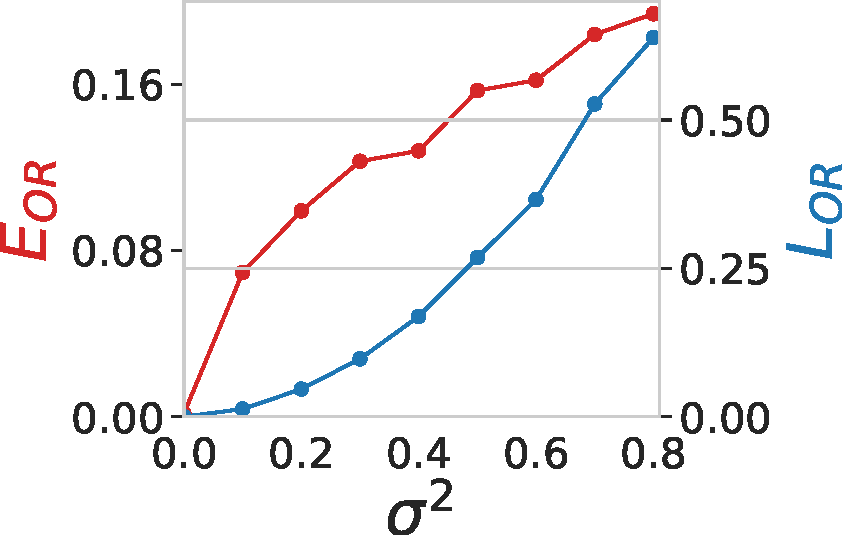
\includegraphics[height=5cm]{figures/5j0n_perfect_noisy_ar_aa}
        \caption{Asymmetric protein (\texttt{5j0n}).}
    \end{subfigure}
    \hfill
    \begin{subfigure}[b]{0.50\linewidth}
    \centering
        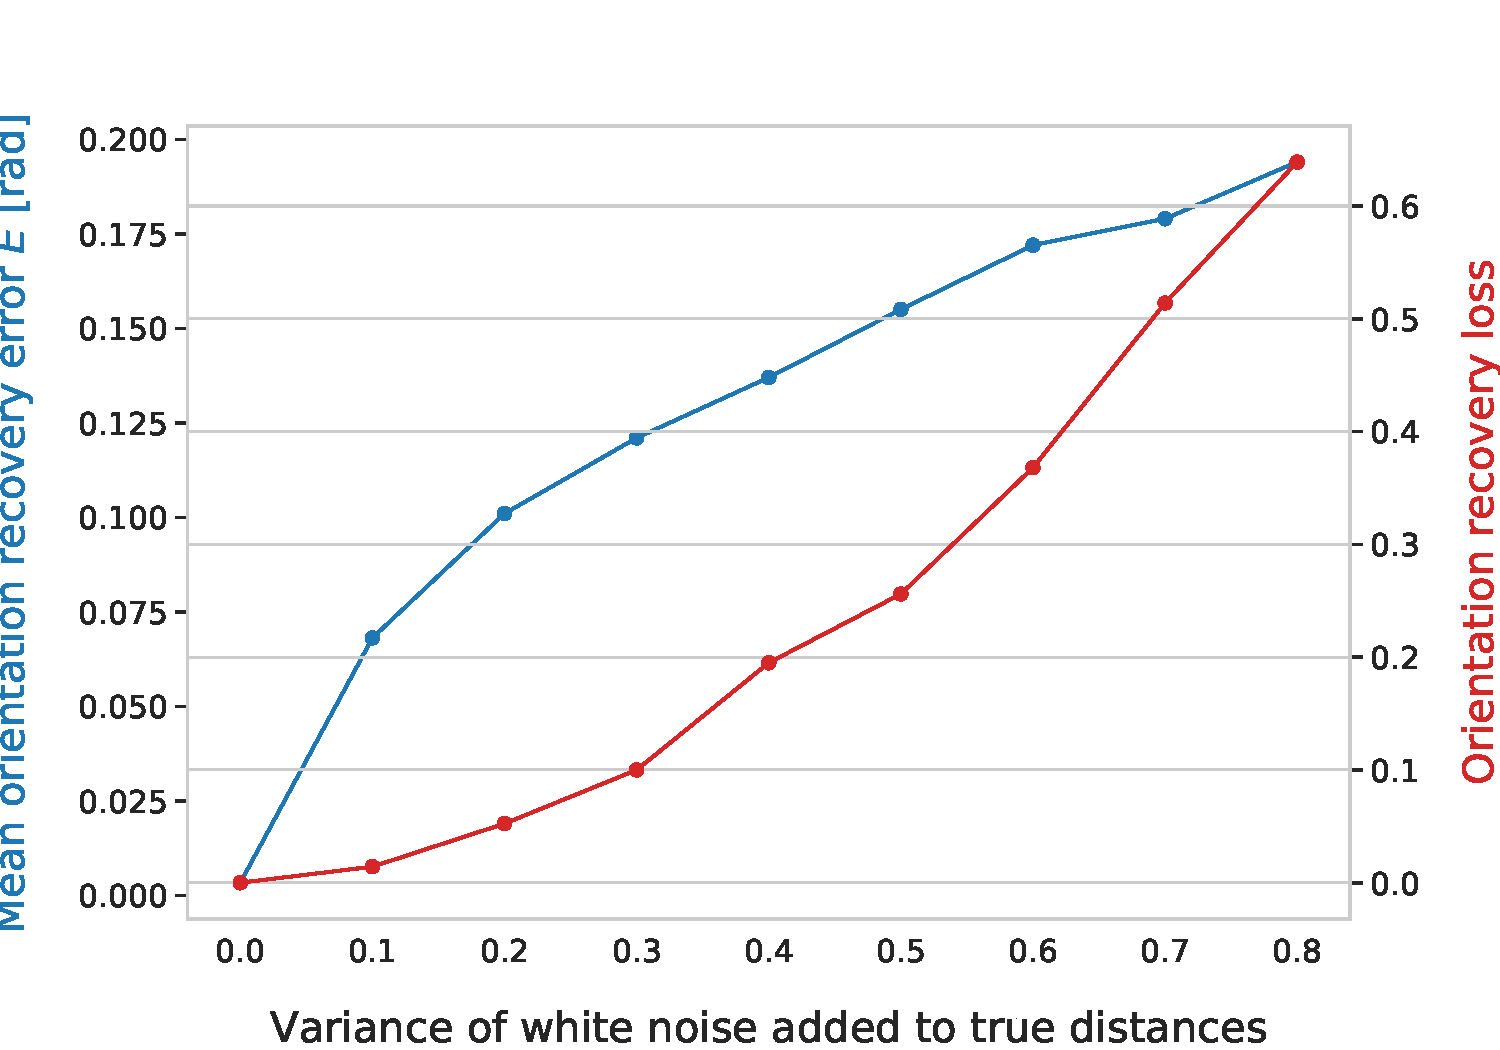
\includegraphics[height=5cm]{figures/5a1a_perfect_noisy_ar_aa}
        \caption{Symmetric protein (\texttt{5a1a}).}
    \end{subfigure}
    \caption{
        The mean orientation recovery error $E$ from \eqnref{orientation-recovery-error} is a monotonic function of the distance estimation error.
        Better distance estimation leads to better orientation recovery.
        Moreover, the recovery loss \eqnref{orientation-recovery} is a good proxy for the recovery error $E$, allowing us to assess recovery performance even without ground-truth orientations.
}
    \label{fig:perfect-with-noise-ar-aa}
\end{figure}

These results demonstrate that the performance of orientation recovery~\eqnref{orientation-recovery} depends on the quality of the estimated distances, which advocates for a proper and extensive training of the SiameseNN in the next stages of development.
Another interesting output of \figref{perfect-with-noise-ar-aa} is that it indicates that the error of the orientation recovery behaves as a monotonic function of its loss.
Hence, it suggests that the loss can be used as a good indicator of its performance, which has obvious practical implications for our future works on real data.

%%%%%%%%%%%%%%%%%%%%%%%%%%%%%%%%%%%%%%%%%%%%%%%%%%%%%%%%%%%%%%%%%%%%%%%%%%%%%%%%%%%%%%%

\subsection{Learned function for relative distance estimation }\label{sec:results:distance-estimation:learned}

%\mdeff{Story: learned distance $d_{ps}$ estimates $d_q$ with some variance but still underestimates larger distances.
%Again symmetric vs asymmetric.}

We present here a preliminary evaluation of the ability of SiameseNNs to learn a projection distance $\widehat{d_p}$ that correctly approximates the orientation distance $d_q$.
To assess the progress and effectiveness of our distance estimation implementation, we used an Euclidean distance as a baseline (see \apxref{results:distance-estimation}).

%SiameseNNs come with a variety of more or less powerful architectures.
%At the current stage of development, we work with a simple one.
%Our SiameseNN is composed of two convolutional neural networks (CNNs) with shared weights.
%Their output features vectors are compared through an Eulidean distance, \textit{i.e.}, $d_f(\mathbf{f}_i,\mathbf{f}_j)=\lVert \mathbf{f}_i-\mathbf{f_j}\rVert_2$ in \figref{schematic:distance-learning}.
%Besides the Euclidean distance, this distance metric $F$ can be defined as geodesic distance, or it could be parametrized as MLP, used for a general function approximation, which we will explore in some of the following experiments.
%\mdeff{Don't repeat what's written in \secref{method:distance-learning}. The general stuff goes there, the specific here.}

\begin{figure}
    \centering
    \begin{subfigure}[t]{0.45\linewidth}
        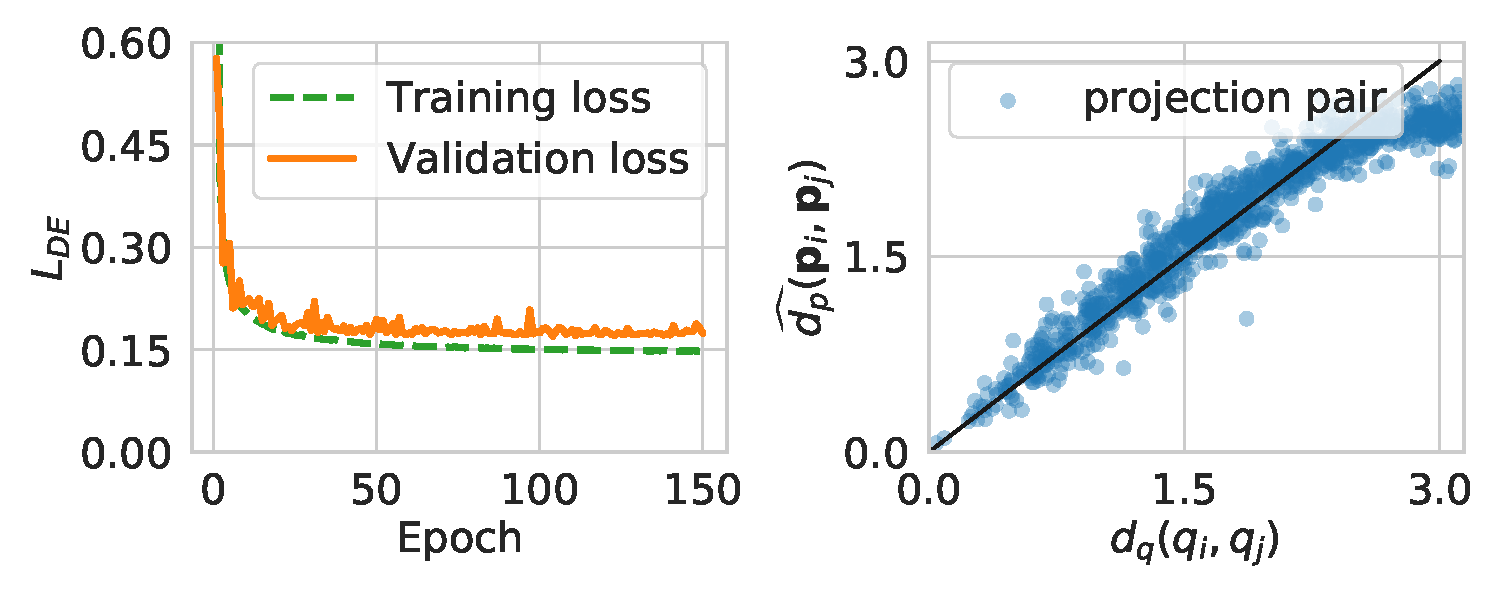
\includegraphics[height=3.5cm]{figures/de_loss_dPdQ_5j0n.pdf}
        \caption{Asymmetric protein (\texttt{5j0n}).}
        \label{fig:losses-siamese-assym}
    \end{subfigure} \quad \quad
    \begin{subfigure}[t]{0.5\linewidth}
        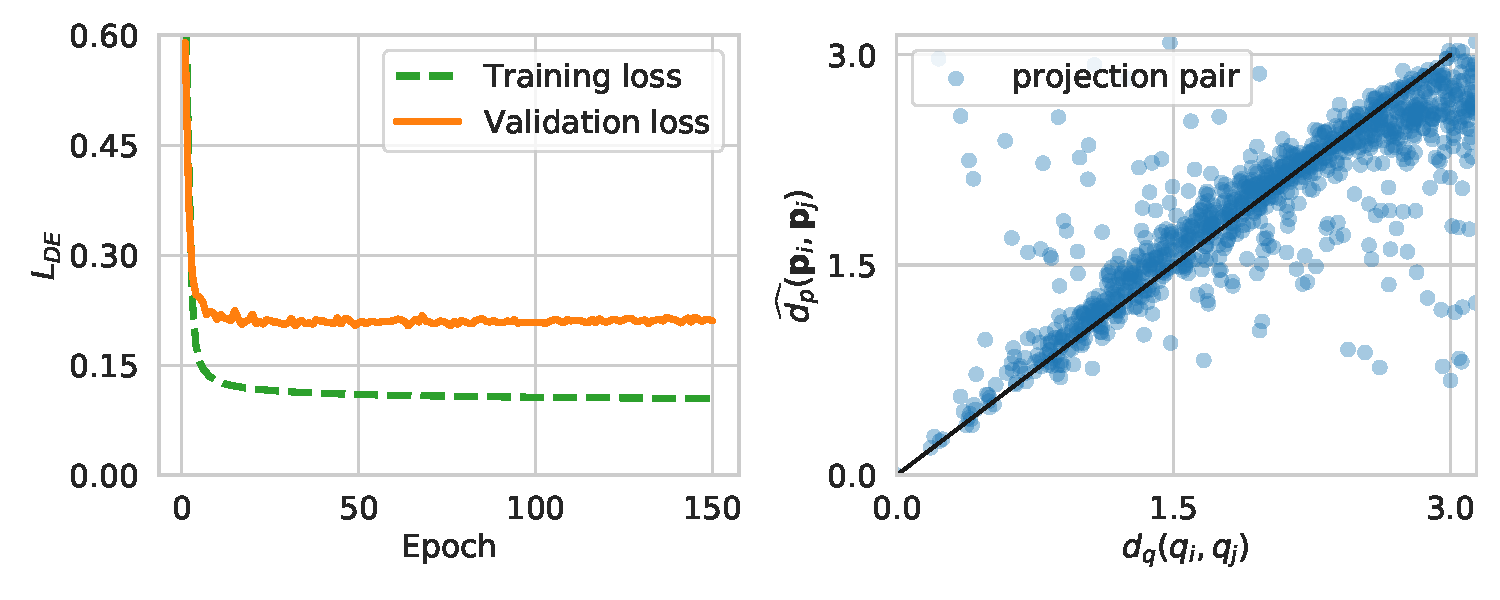
\includegraphics[height=3.5cm]{figures/de_loss_dPdQ_5a1a.pdf}
        \caption{Symmetric protein (\texttt{5a1a}).}
        \label{fig:losses-siamese-sym}
    \end{subfigure}
    \caption{
        Distance learning loss \eqnref{distance-learning} evaluated on the training and validation datasets during learning/training (on the left side respectively). Relationship between orientations' distance $d_q$ and estimated distance $d_p$ on the test dataset (on the right side respectively).
    }\label{fig:losses-siamese}
\end{figure}

% \begin{figure}
%     \centering
%     \begin{subfigure}[b]{0.5\columnwidth}
%         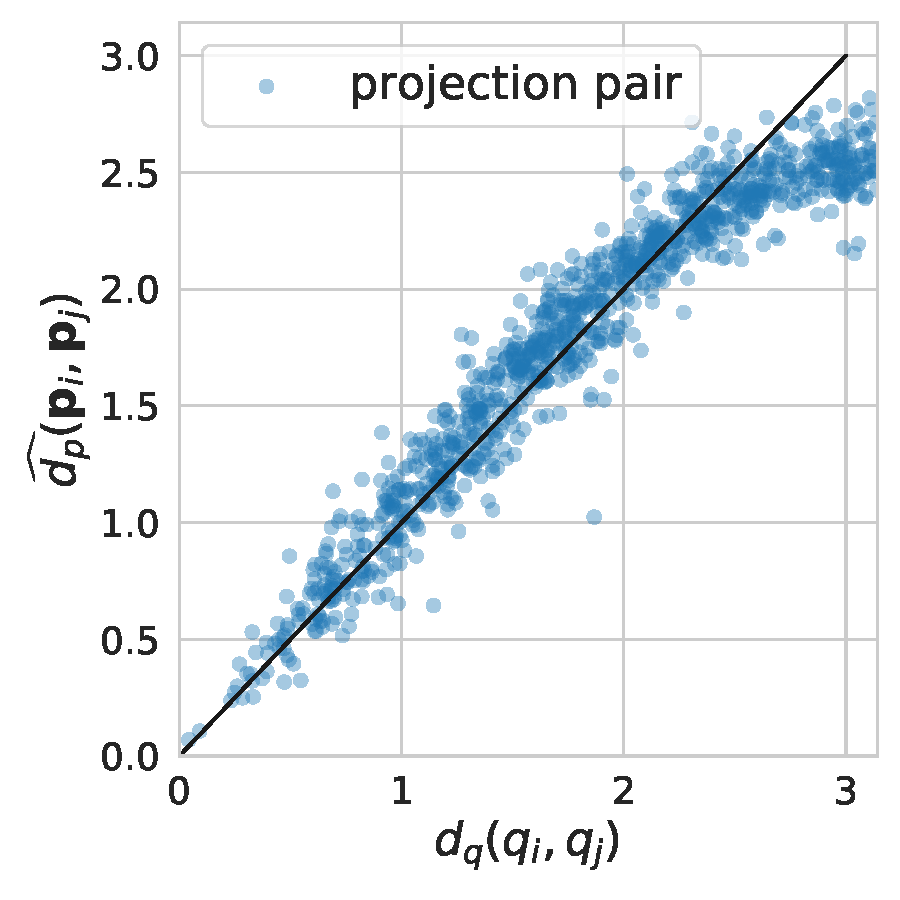
\includegraphics[height=6cm]{figures/dPdQ_5j0n}
%         \caption{Asymmetric protein (\texttt{5j0n}) on test dataset.}
%     \end{subfigure}
%     %\hfill
%     \begin{subfigure}[b]{0.45\columnwidth}
%     \centering
%         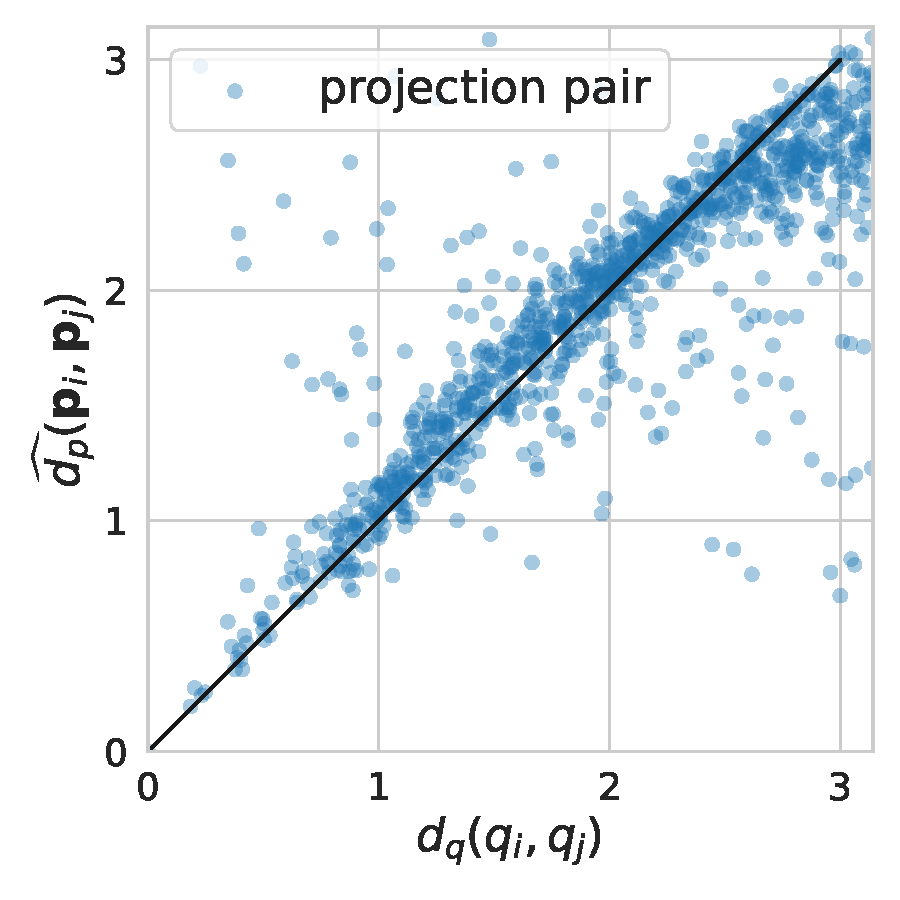
\includegraphics[height=6cm]{figures/dPdQ_5a1a}
%         \caption{Symmetric protein (\texttt{5a1a}) on test dataset.}
%     \end{subfigure}
%     \caption{Relationship between orientations' distance $d_q$ and estimated distance $d_p$.}
%     \label{fig:learned-distance-siamese}
% \end{figure}

As a feature distance $d_f$ between the outputs of the two CNNs we used the Geodesic distance \eqnref{geodesic-distance}.
\mdeff{We wrote in the method that we take $d_f=d_q$. Shall we repeat? I don't think we should if the only experiments where that is untrue is in \apxref{feature-distance}.}
The pairs for the training were sampled from $1\%$ of maximum number of training pairs $P_{\text{train}}^2$ ($63,126$ pairs) and validation was performed on $1\%$ of the maximum number of validation pairs $P_{\text{val}}^2$ ($27,225$ pairs).
We limited our training and validation dataset due to Google Colaboratory\footnote{A hosted Jupyter notebook service from Google Research with resources that are not guaranteed and not unlimited.} training time limit of 12 hours.

%\mdeff{So those pairs are sampled from $63,126$ pairs from the training dataset, rather than the $P^2$ possible pairs? If true, we should motivate somewhere why we limit our training dataset.}
Depending on the available resources on the Google Colaboratory, the training lasted from 2.6 hours to 9.3 hours on one of its GPUs.
The evolution of the training and validation losses are presented on the left side in \figref{losses-siamese-assym} for the asymmetric protein (\texttt{5j0n}), and on the left side in \figref{losses-siamese-sym} for the symmetric one (\texttt{5a1a}).
The results demonstrate that the SiameseNN succeeded at learning a proxy distance for the asymmetric protein dataset, as convergence was reached in about 50 epochs ($\sim$ 50 minutes in the best resource availability setting).

Similarly to Euclidean distance $d_p$, we noticed that the larger distances $d_q$ were poorly predicted and the plot again had a slight plateau phenomenon for the distances higher than~$2.5$ rad.
\mdeff{Insist that this is much better than Euclidean $d_p$.}
\mdeff{Future work: fix or downplay the influence of larger distances in orientation recovery.}

It is interesting to see that both validation losses were around $0.2$.
However, the current SiameseNN architecture slightly overfits at learning the distance for the dataset \texttt{5a1a}, which is very likely due to the symmetry of the $\beta$-galactosidase protein, even thought the quarter-sphere coverage was used.
%Indeed, its synthetic dataset may still contain pairs of projections that share the same $d_p$, yet differ in their $d_q$.
This simply advocates for the restriction to non-overlapping areas on $\SO(3)$ when sampling the orientations used to generate the SiameseNN training dataset.
The latter would then only contain projection pairs with a linear $(d_q,d_p)$ relationship, which should ensure a successful training of the network.
%\mdeff{I don't get this explanation. Do you mean that \texttt{5a1a} might have other symmetries than D2?}
For the rest of the experiments, we used the asymmetric protein (\texttt{5j0n}) dataset.
Besides using the asymmetric protein, we performed the full protein reconstruction pipeline on the symmetric protein (\texttt{5a1a}).

We then fed to the trained SiameseNN $1,000$ pairs of projections randomly selected from the \texttt{5j0n} testing dataset, and reported the $(d_q,\widehat{d_p})$ relationship of each pair in \figref{losses-siamese} (right side of each subfigure).
These results confirm that, the SiameseNN was able to predict the orientation distance $d_q$ using only the projections as inputs.
The prediction performance was slightly better for the asymmetric protein compared to symmetric protein.
Moreover, it clearly outperformed the Euclidean distance at doing so.
These preliminary results are encouraging, as much has yet to be gained from improving upon the rather primitive SiameseNN architecture we currently use.
The architecture of implemented SiameseNN can be seen in \apxref{siamese-architecture}.
Besides concentrating on the hyperparameter selection and tuning of the neural network layers, we also evaluated the performance of the model depending on the feature distance we used for the SiameseNN, see \figref{geo-eucl-mlp} and \apxref{feature-distance}.

%%%%%%%%%%%%%%%%%%%%%%%%%%%%%%%%%%%%%%%%%%%%%%%%%%%%%%%%%%%%%%%%%%%%%%%%%%%%%%%%%%%%%%%

\subsection{Sensitivity of distance learning to perturbations in the projections}\label{sec:results:distance-estimation:sensitivity}
%\subsection{Generalization of distance learning}
%\subsection{Generalizability/Abstractability of distance learning}

%\mdeff{Story: learned distance is minimally sensible to perturbations (additive noise, translation, PSF) because we can train it to ignore irrelevant information.
%Thanks again to good model of cryo-EM imaging.}
%\mdeff{Better word? (perturbations, corruptions, quality, non-ideal)}

% Intro and shift.
We desire to estimate distances that are invariant to perturbations in the projections---specified in~\eqnref{imaging-model}.
As discussed in \secref{method:distance-learning}, the convolutional architecture of the SiameseNN should be shift invariant.
\figref{results:distance-estimation:shift} indeed shows that learning distances (and hence recovering orientations) is insensible to shifts in projections.

% Noise.
As we cannot---or do not (yet) know how to---build noise invariance into the architecture, we trained the SiameseNN on noisy datasets and evaluated whether it could learn to ignore noise as being irrelevant information.
% brute force vs principled engineering
\figref{results:distance-estimation:noise} shows a mean orientation recovery error of $E_\text{OR} \approx 0.16$ radians ($\approx 9\degree$) for noiseless projections and $E_\text{OR} \approx 0.42$ radians ($\approx 24\degree$) for a more realistic noise variance of $\sigma^2=15$.
\mdeff{How good is that?}
While a naive distance function (like an Euclidean distance) would be tremendously sensitive to noise, the SiameseNN mostly learned to discard it.
Moreover, overfitting (i.e., the growing gap between the validation and trainig losses) indicates that more training data will further decrease the SiameseNN's sensitivity to noise.

% PSF and conclusion.
We didn't evaluate sensitivity to the PSF but expect a similar behavior.
%While we would ideally want the NN architecture to be engineered to ignore irrelevant information, that is not always possible.
%We know how to do it for shifts, not noise or PSF.

We observe that the estimation of more accurate distances (a smaller $L_\text{DE}$) leads to the recovery of more accurate orientations (a smaller $L_\text{OR}$ and $E_\text{OR}$).
Moreover, we observe again (\secref{results:orientation-recovery:sensitivity}) that an higher recovery loss $L_\text{OR}$ induces an higher error $E_\text{OR}$.

%\subsection{Estimating distances on unseen proteins}

As the SiameseNN will ultimately be trained on known proteins and used to estimate distances on unknown proteins to be imaged,
%we also desire our learned distance function to generalize/transfer across density maps $\x$.
we also desire our learned distance function to generalize to unseen proteins.
The distance function $\widehat{d_p}$ must abstract the protein (in the same way it must abstract shifts, noise, or PSFs to generalize to unseen projections).
\mdeff{Noiseless for all proteins right?}
We attempted to recover the orientations of projections from \texttt{5j0n} while we had trained the SiameseNN on four other proteins (\texttt{5nvu}~\cite{5nvu_pdb}, \texttt{5nvs}~\cite{5nvs_pdb}, \texttt{6mem}~\cite{6mem_pdb}, \texttt{6o1o}~\cite{6o1o_pdb} \todo{should be the same ``kind'' of refs as the ones used in 3.1 for \texttt{5j0n} and \texttt{5a1a}}, which have the same type of symmetry as \texttt{5j0n}).
\todo{Same number of projections as in \tabref{dataset}?}
We obtained a recovery loss of $L_\text{OR} = 0.0352$ \mdeff{Could we also have $E_\text{OR}$? It's easier to understand and compare.},
to be compared with $L_\text{OR} \approx 0.11$ when the SiameseNN was trained on \texttt{5j0n} alone.
While performance is somewhat degraded, we conclude that it is possible to use a learned distance function on unseen proteins.

\begin{figure}[ht!]
    \centering
    \begin{subfigure}[t]{0.47\linewidth}
        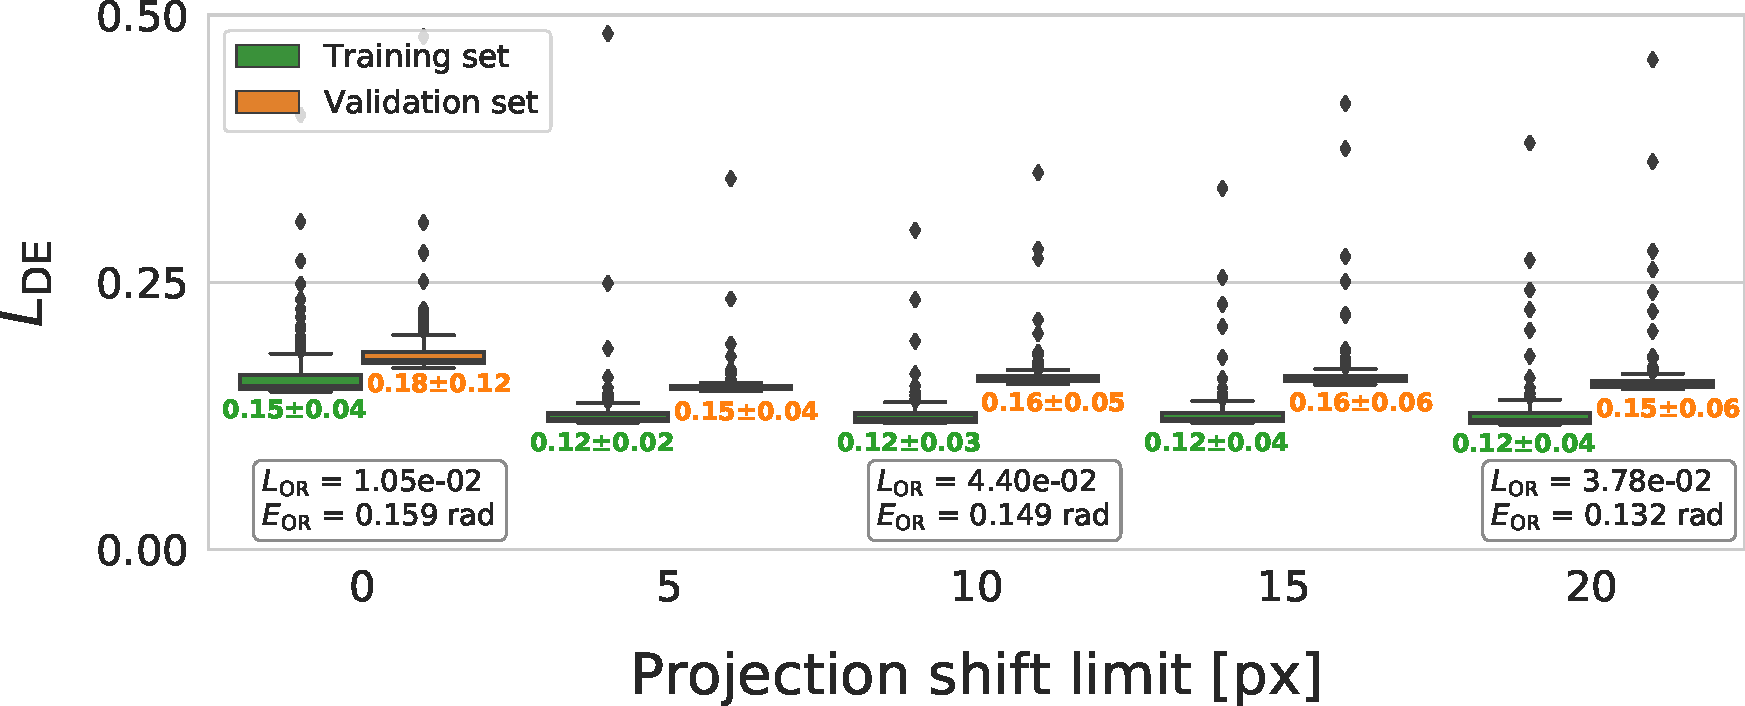
\includegraphics[width=\linewidth]{figures/de_translation_nums}
        \caption{%
            Learning from shifted projections $\{ \mathbf{S}_{\mathbf{t}_i} \mathbf{P}_{\bth_i} \mathbf{x} \}$, with translations $t_{i_1}$ and $t_{i_2}$ sampled from a triangular distribution with mean 0 and of increasing limits.
            Learning is not harder as projections get shifted farther, because shift invariance is built into the convolutional architecture of $\mathcal{G}_w$.
    }\label{fig:results:distance-estimation:shift}
    \end{subfigure}
    \hfill
    \begin{subfigure}[t]{0.47\linewidth}
        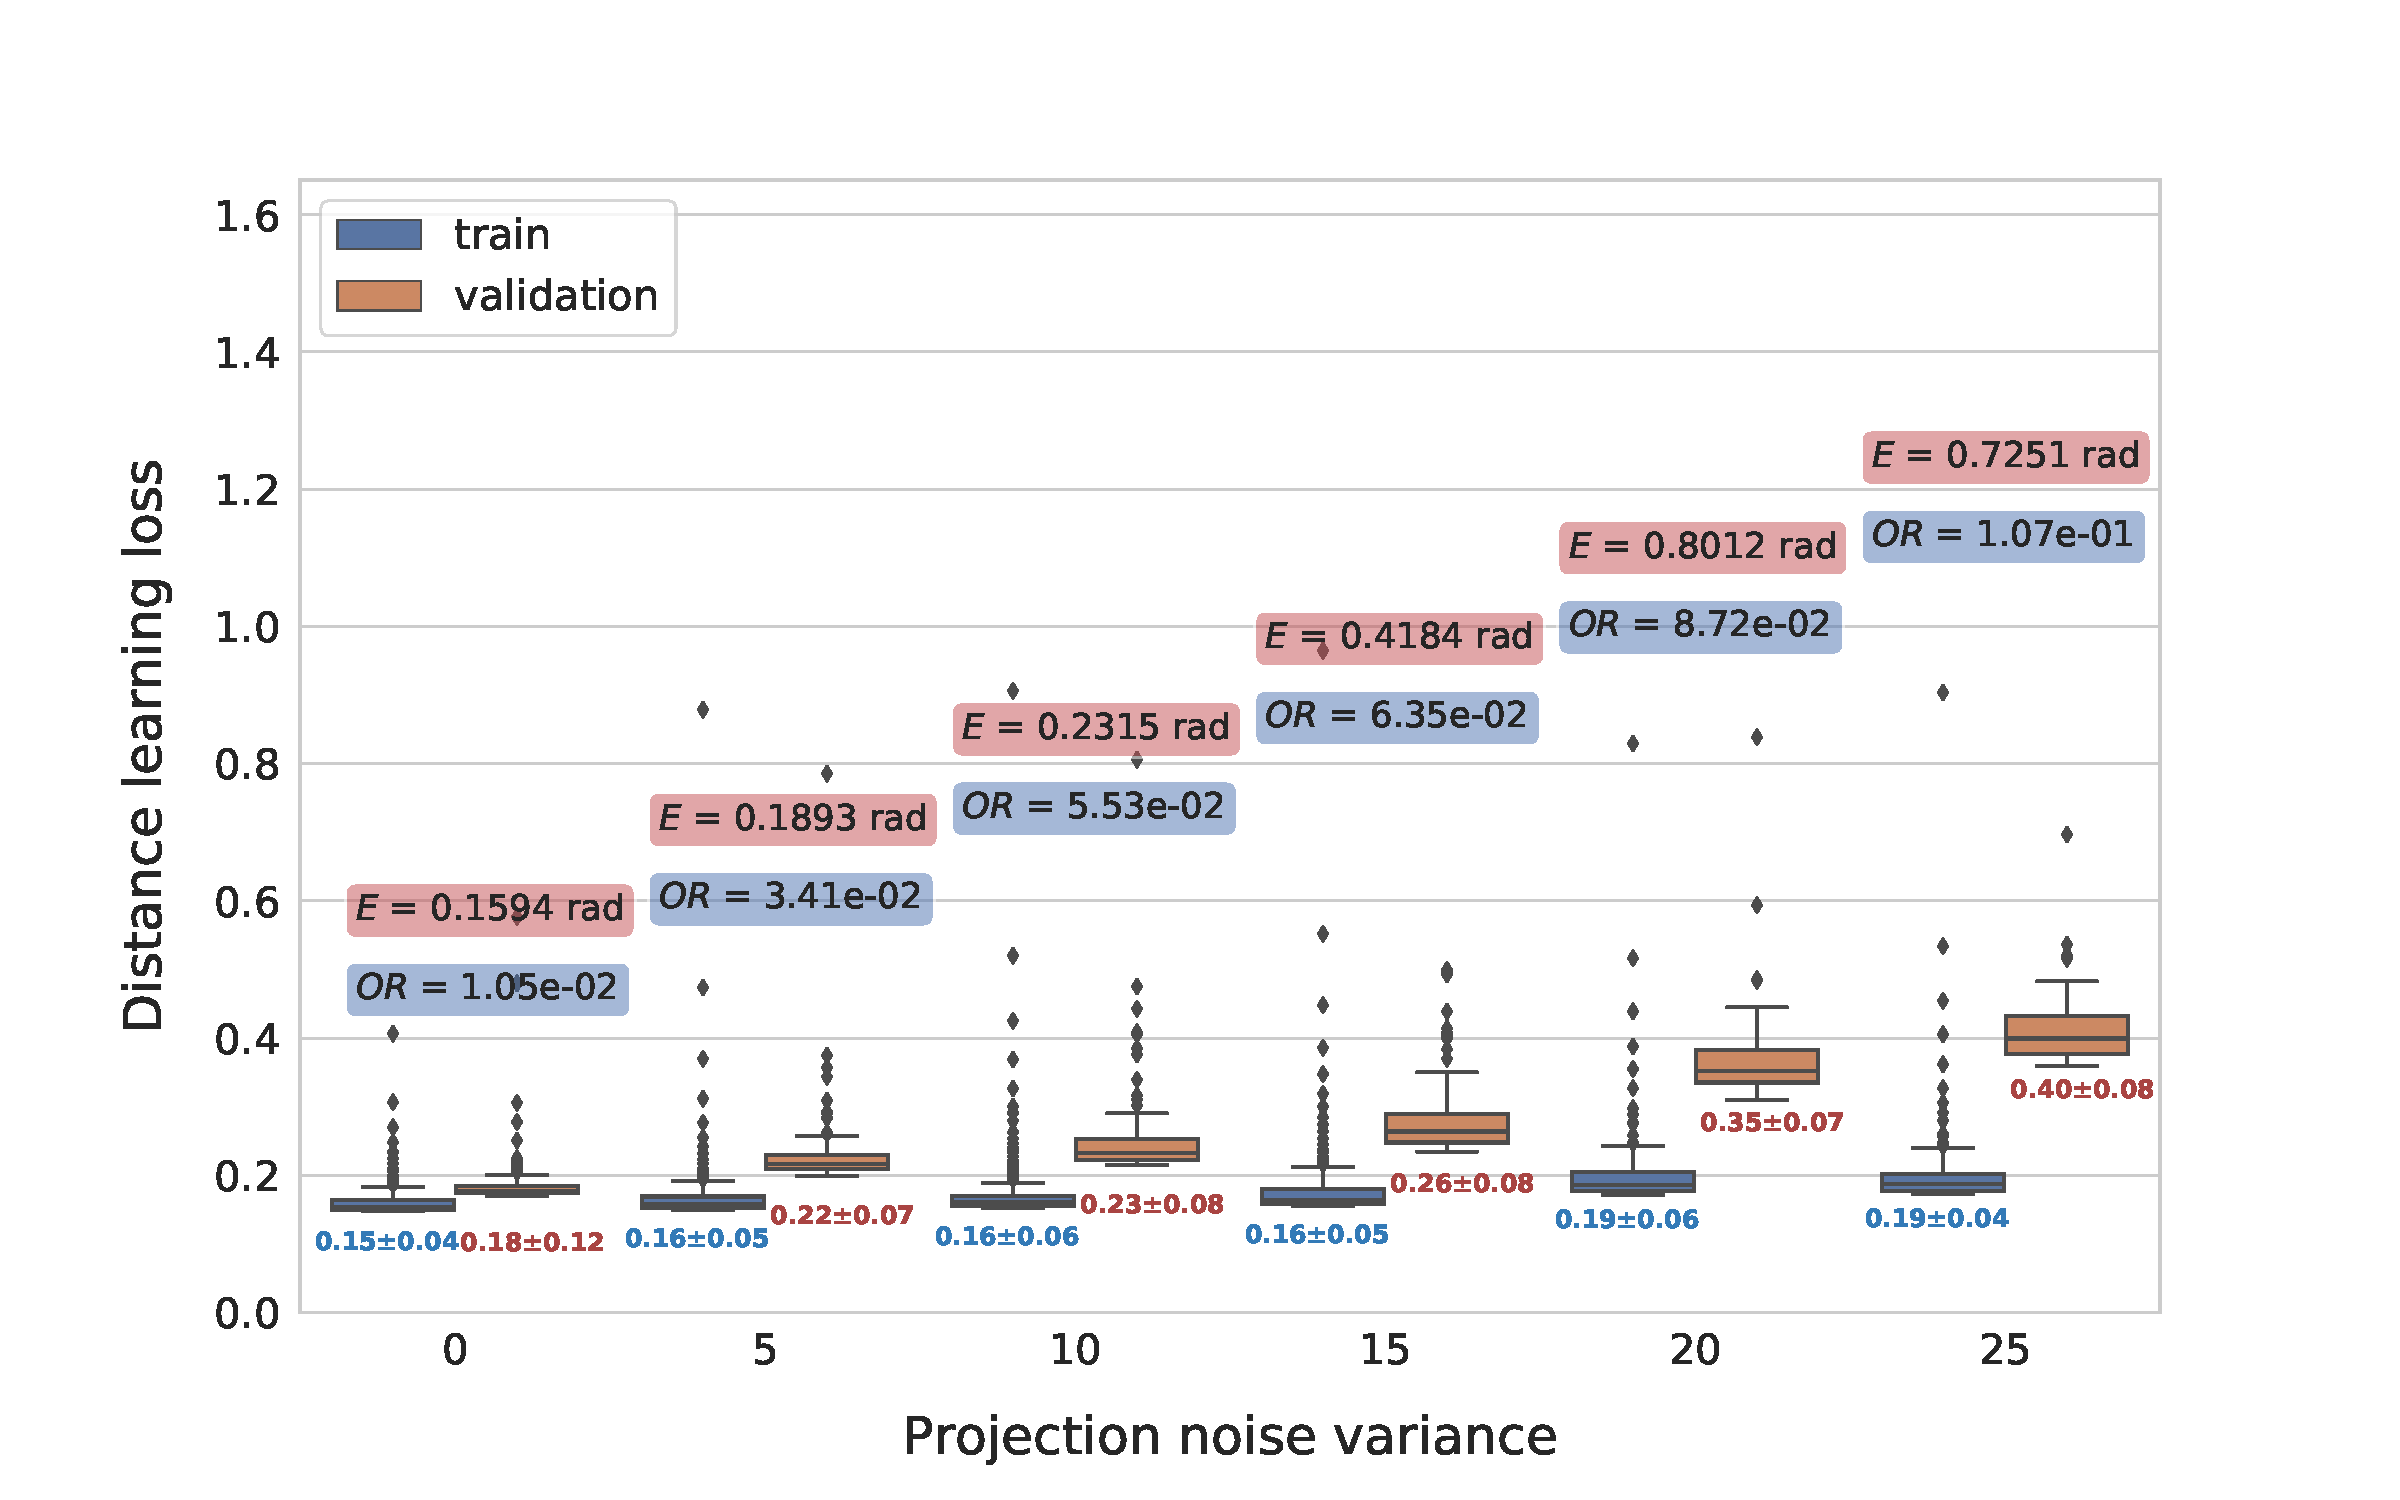
\includegraphics[width=\linewidth]{figures/de_noises_nums}
        \caption{%
            Learning from noisy projections $\{ \mathbf{P}_{\bth_i} \mathbf{x} + \mathbf{n} \}$, with white noise $\mathbf{n} \sim \mathcal{N}(0, \sigma^2\mathbf{I})$ of increasing variance $\sigma^2$.
            Learning is harder as projections get noisier, because noise invariance is not built into the architecture of $\mathcal{G}_w$.
        }\label{fig:results:distance-estimation:noise}
    \end{subfigure}
    \caption{%
        Sensitivity of distance learning to perturbations in the projections of \texttt{5j0n}.
        The box plots show the distance learning loss $L_\text{DE}$ \eqnref{distance-learning} on the training (blue) and validation (red) sets.
        \mdeff{Numbers are per pair or per batch of 256 pairs?}
        Boxes show the orientation recovery loss $L_\text{OR}$ \eqnref{orientation-recovery} and error $E_\text{OR}$ \eqnref{orientation-recovery-error}.
        \mdeff{It's confusing that red and blue are used for both train vs validation and $E_\text{OR}$ vs $L_\text{OR}$. I don't think we need colors for $E_\text{OR}$ and $L_\text{OR}$. They could both be in the same black box.}
        \todo{Legend consistency: train -> training set, validation -> validation set.}
        \todo{Add $L_\text{DE}$ to the y-axis legend.}
        \todo{Add $\sigma^2$ to the x-axis legend of (b).}
    }
\end{figure}

%%%%%%%%%%%%%%%%%%%%%%%%%%%%%%%%%%%%%%%%%%%%%%%%%%%%%%%%%%%%%%%%%%%%%%%%%%%%%%%%%%%%%%%

\subsection{Orientation recovery and density reconstruction from estimated distances}\label{sec:results:orientation-recovery:reconstruction}
%\subsection{Density reconstruction from recovered orientations}

\todo{
\begin{itemize}
    \item Make the plots in Figures~\ref{fig:5j0n-noise0-orientation-recovery},~\ref{fig:5j0n-noise16-orientation-recovery}, and~\ref{fig:5a1a-noise0-orientation-recovery} flatter and remove \texttt{width=linewidth} (which deforms the figure).
    \item Add $L_\text{OR}=...$ and $E_\text{OR}=...$ in the boxes of Figures~\ref{fig:5j0n-noise0-orientation-recovery},~\ref{fig:5j0n-noise16-orientation-recovery}, and~\ref{fig:5a1a-noise0-orientation-recovery}.
    \item Would be nice to know $L_\text{DE}$ for the three cases.
    \item ``With total of $1,650$ projections in the test dataset, we were able to reconstruct the protein.'' \mdeff{But \tabref{dataset} says 838 for test. Was it validation data?}
    \item \mdeff{Training set for distance learning and validation/test set for orientation recovery should have been made clear in 3.1.}
\end{itemize}
}

As a proof-of-concept, we attempted to solve the inverse problem posed by \eqnref{imaging-model}.
We reconstructed density maps $\widehat{\x}$ from sets of projections $\{ \p_i \}$ and their orientations $\{ \widehat{q_i} \}$ as recovered by our method.
%We ran the full pipeline---distance estimation, orientation recovery, and protein reconstruction---to validate our method.
%The orientation recovery from estimated distances represents a full pipeline needed to reconstruct the protein from a given set of projections.
Note that we only trained the SiameseNN \eqnref{distance-learning} on projections from the protein (and noise level) we attempted to reconstruct from.
For best performance, it should be trained on multiple proteins, levels of noise, PSFs, etc.

To understand the effect of miss-recovered orientations, we reconstructed the density maps from both the recovered orientations $\{ \widehat{q_i} \}$ and the true orientations $\{ q_i \}$ along which the projections $\{ \p_i \}$ were acquired.
The density maps were reconstructed by the ASTRA toolbox.
\todo{Using the ASTRA toolbox, we generated orientation vectors based on angles which we fed into projection 3D geometry in ASTRA.}
\todo{Make clearer. Are there enough details?}
\mdeff{Laurène, could you write something about how ASTRA is a naive reconstruction method (compared to the SOTA discussed in the intro), and that we did it only to get a crude idea? Or something along those lines. ;)}
For an unknown reason, we had to align the recovered orientations with \eqnref{orientation-recovery-error} before feeding them to ASTRA.
\todo{More details. What happened otherwise? We want to say it's an ASTRA issue not something with our method.}

\begin{figure}[t]
    \centering
    \begin{subfigure}[b]{0.44\linewidth}
        \centering
        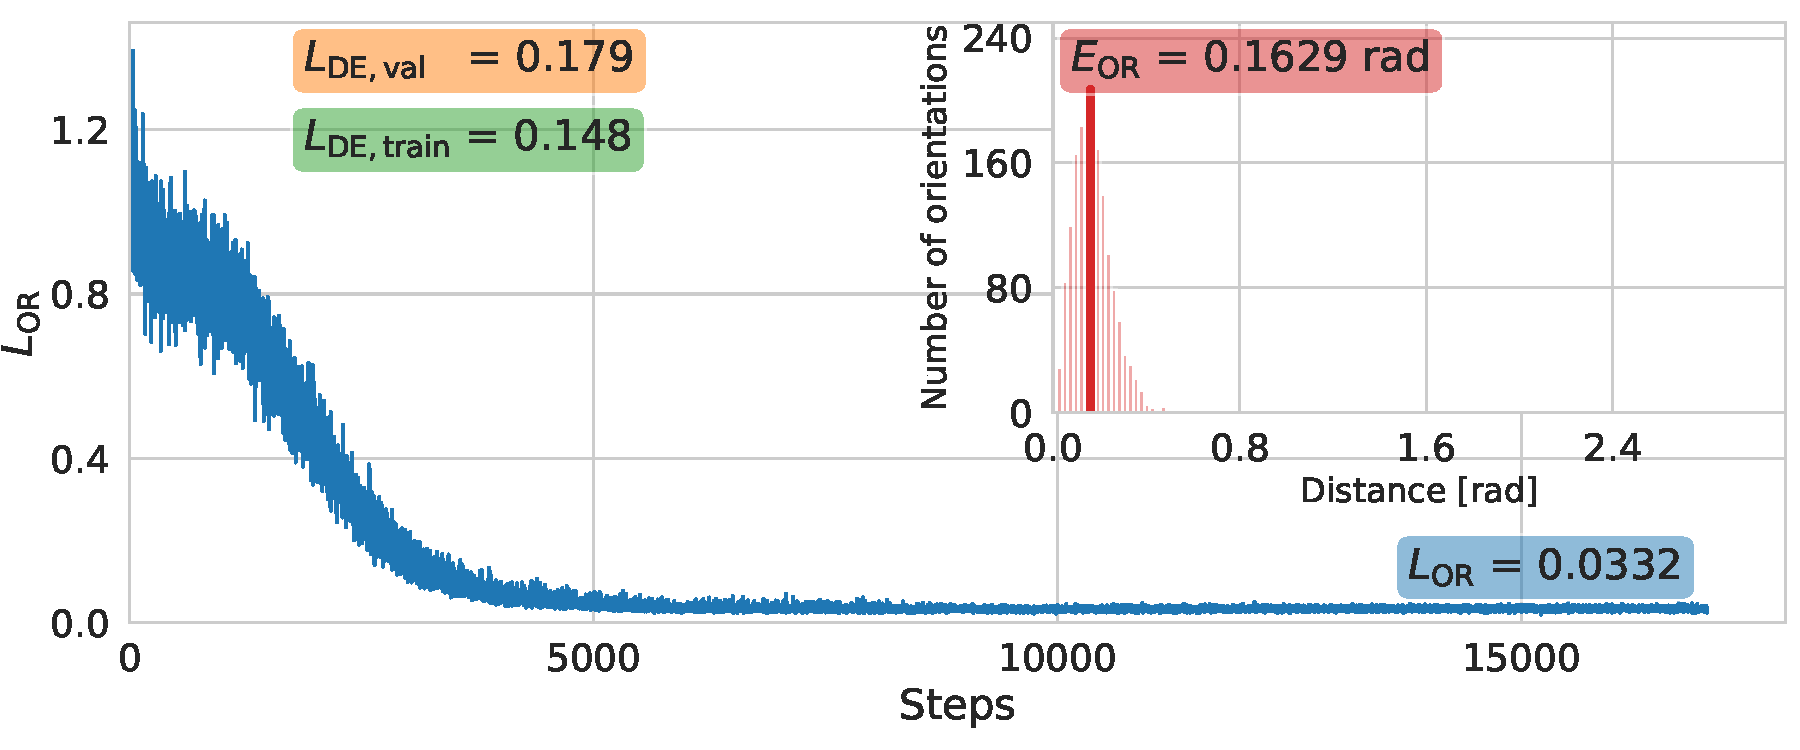
\includegraphics[width=\linewidth,height=8em]{figures/5j0n_noise0_ar_aa}
        \caption{Recovered $\{ \widehat{q_i} \}$ from $\{ \p_i = \mathbf{P}_{\bth_i} \x \}$, $\x$ from \texttt{5j0n}.}%
        \label{fig:5j0n-noise0-orientation-recovery}
    \end{subfigure}
    \hfill
    \begin{subfigure}[b]{0.26\linewidth}
        \centering
        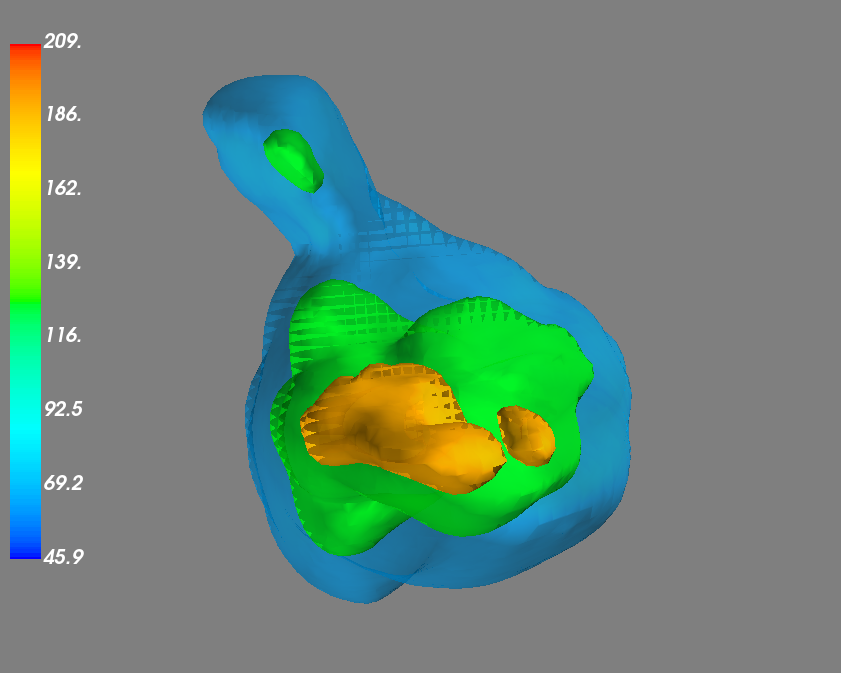
\includegraphics[height=8em]{figures/5j0n_reconstruction_noise0}
        \caption{Reconstructed $\widehat{\x}$ from $\{ \p_i, \widehat{q_i} \}$.}%
        \label{fig:5j0n-noise0-reconstruction-recovered}
    \end{subfigure}
    \hfill
    \begin{subfigure}[b]{0.26\linewidth}
        \centering
        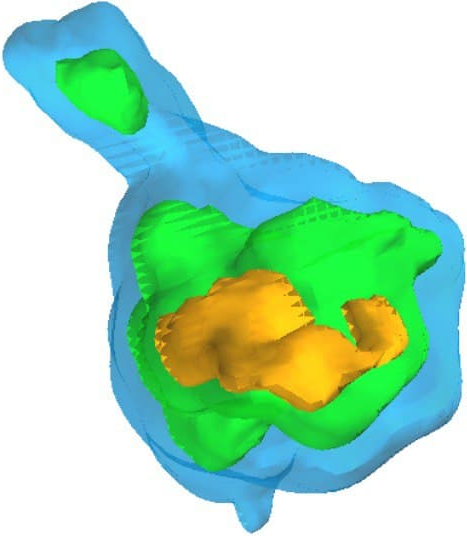
\includegraphics[height=8em]{figures/5j0n_reconstruction_GT}
        \caption{Reconstructed $\widehat{\x}$ from $\{ \p_i, q_i \}$.}%
        \label{fig:5j0n-noise0-reconstruction-true}
    \end{subfigure}
    \\ \vspace{1em}
    \begin{subfigure}[b]{0.44\linewidth}
        \centering
        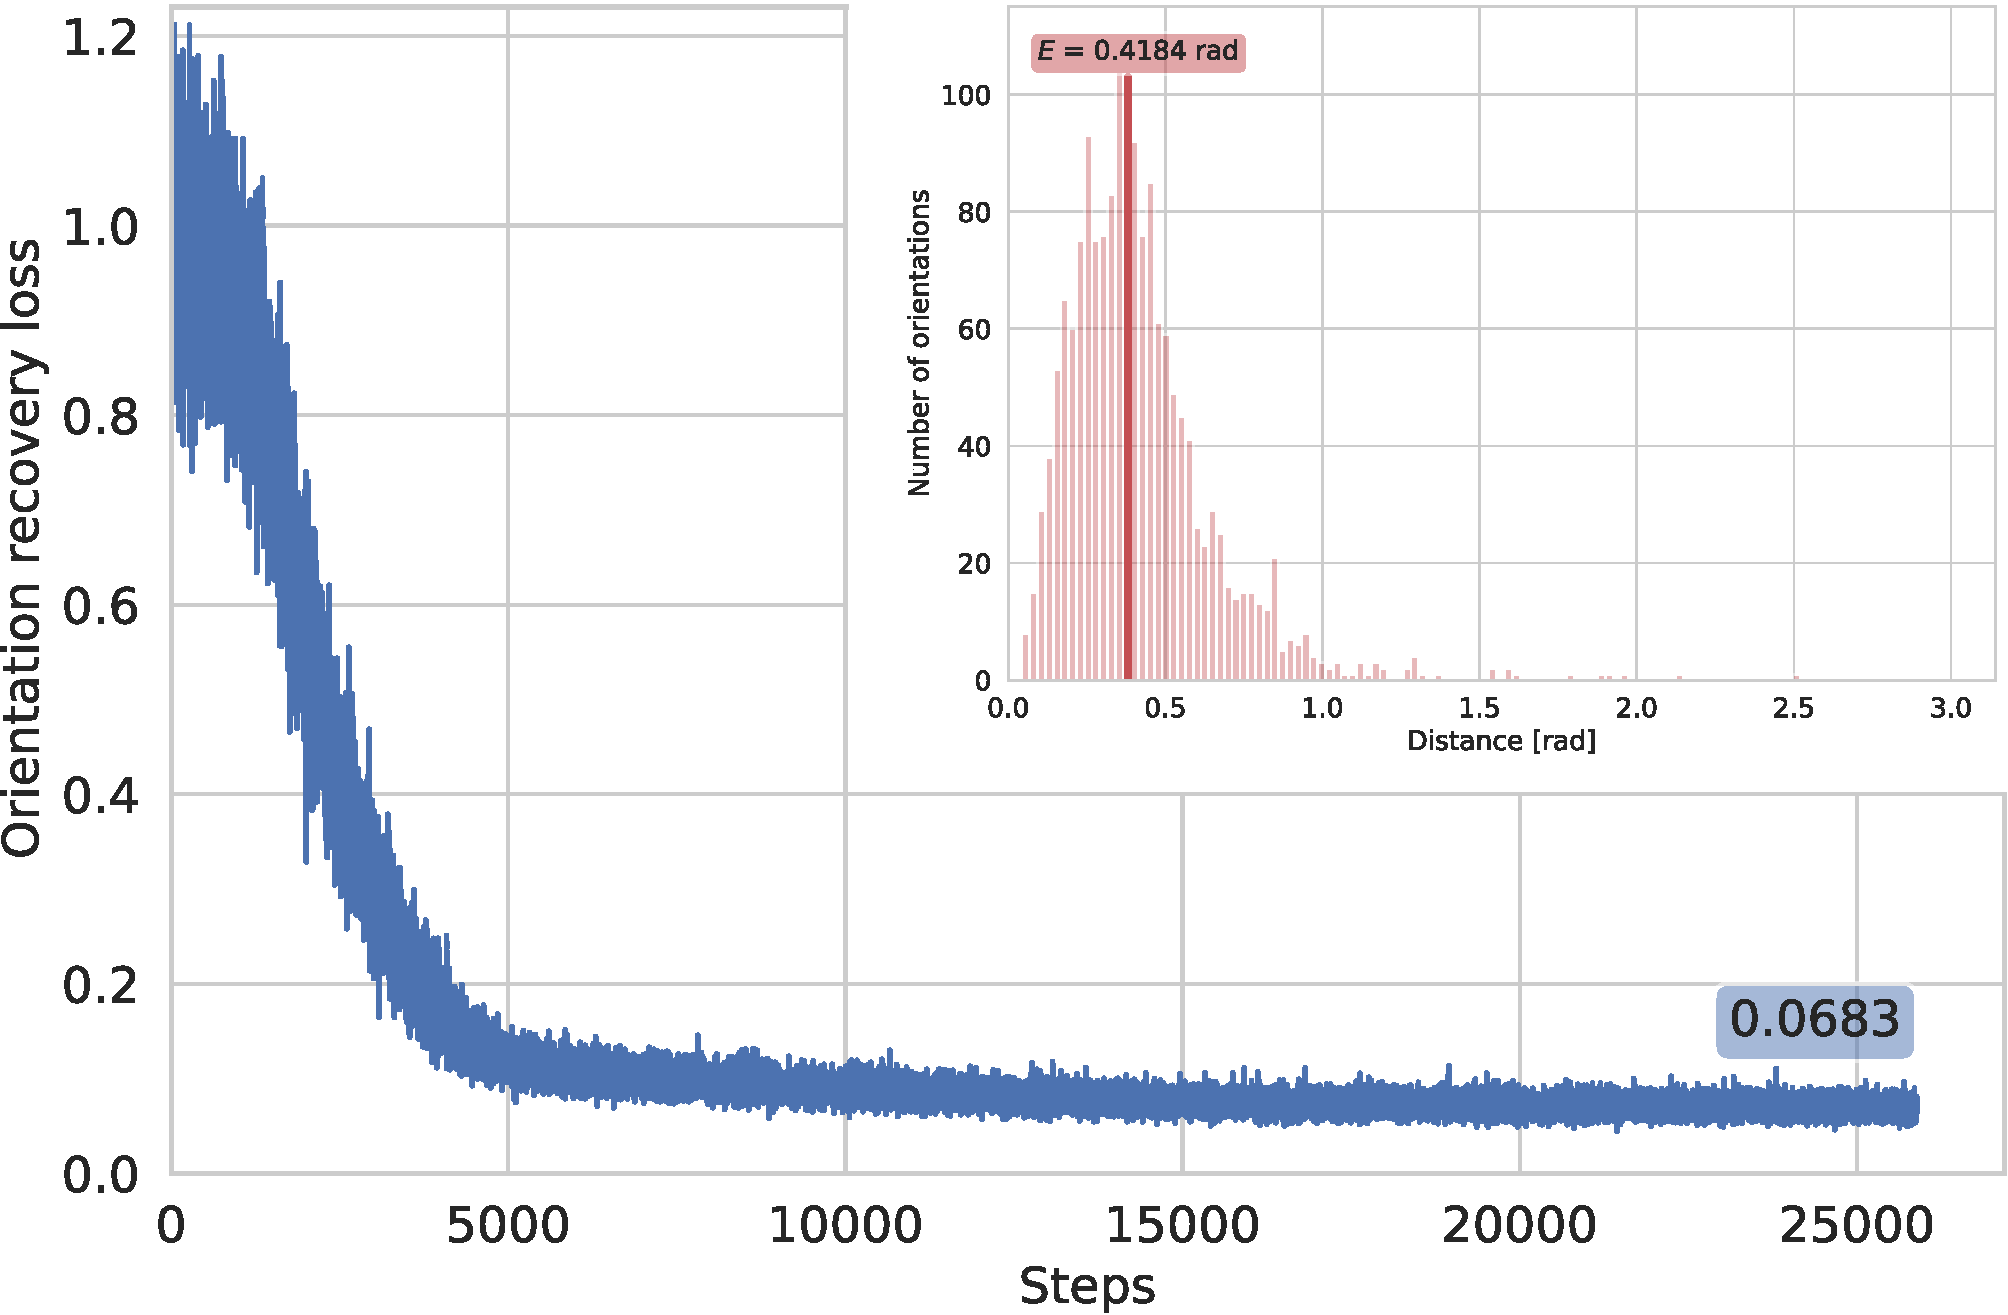
\includegraphics[width=\linewidth,height=8em]{figures/5j0n_noise16_ar_aa}
        \caption{Recovered $\{ \widehat{q_i} \}$ from $\{ \p_i = \mathbf{P}_{\bth_i} \x + \mathbf{n} \}$, $\x$ from \texttt{5j0n}.}%
        \label{fig:5j0n-noise16-orientation-recovery}
    \end{subfigure}
    \hfill
    \begin{subfigure}[b]{0.26\linewidth}
        \centering
        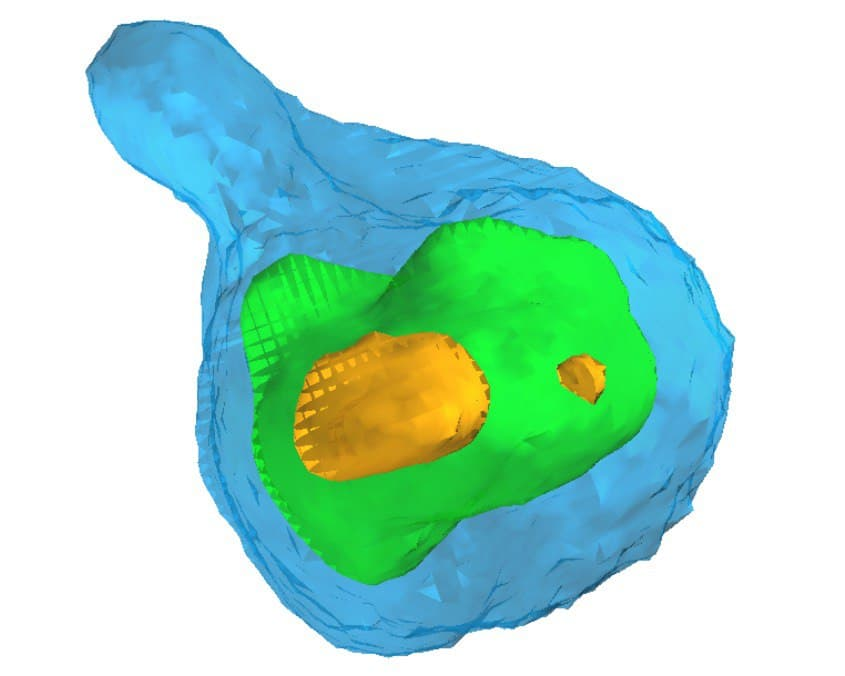
\includegraphics[height=8em]{figures/5j0n_reconstruction_noise16}
        \caption{Reconstructed $\widehat{\x}$ from $\{ \p_i, \widehat{q_i} \}$.}%
        \label{fig:5j0n-noise16-reconstruction-recovered}
    \end{subfigure}
    \hfill
    \begin{subfigure}[b]{0.26\linewidth}
        \centering
        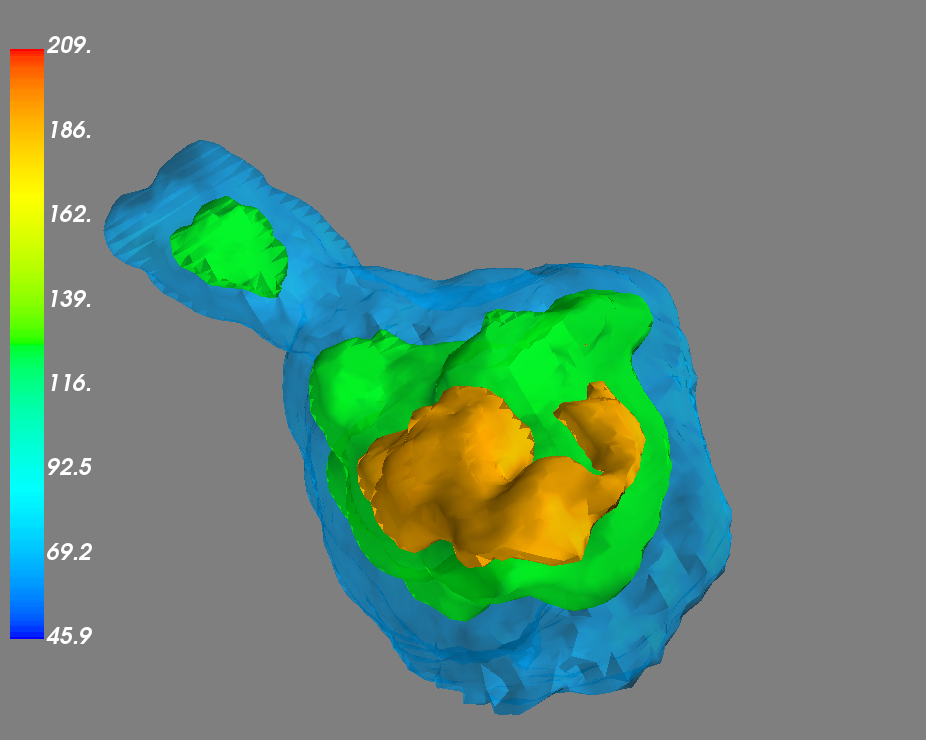
\includegraphics[height=8em]{figures/5j0n_reconstruction_GT_noise16}
        \caption{Reconstructed $\widehat{\x}$ from $\{ \p_i, q_i \}$.}%
        \label{fig:5j0n-noise16-reconstruction-true}
    \end{subfigure}
    \\ \vspace{1em}
    \begin{subfigure}[b]{0.44\linewidth}
        \centering
        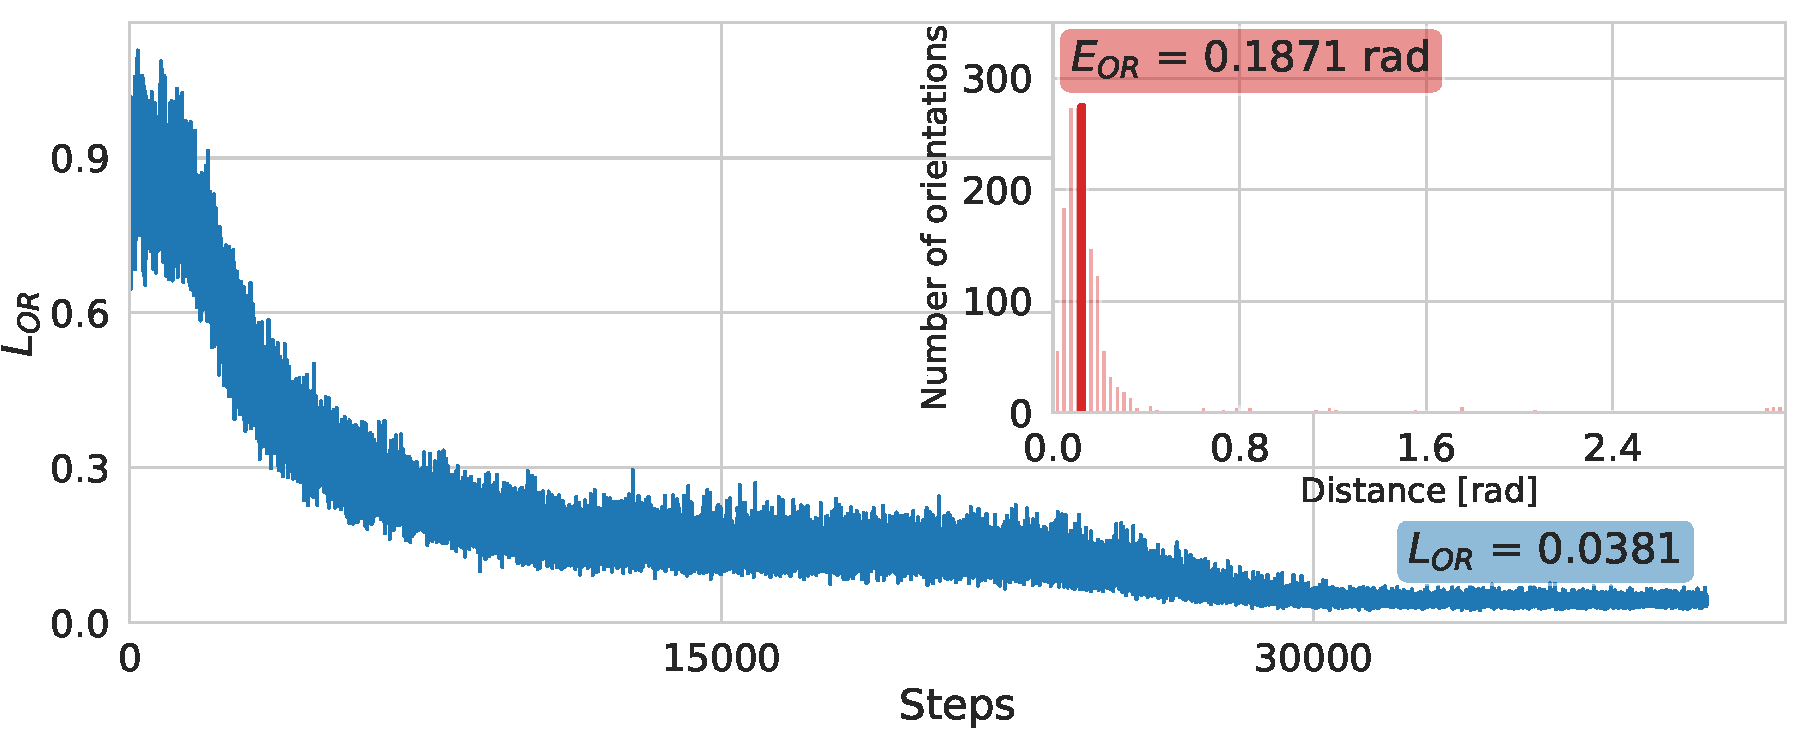
\includegraphics[width=\linewidth,height=8em]{figures/5a1a_noise0_ar_aa}
        \caption{Recovered $\{ \widehat{q_i} \}$ from $\{ \p_i = \mathbf{P}_{\bth_i} \x \}$, $\x$ from \texttt{5a1a}.}%
        \label{fig:5a1a-noise0-orientation-recovery}
    \end{subfigure}
    \hfill
    \begin{subfigure}[b]{0.26\linewidth}
        \centering
        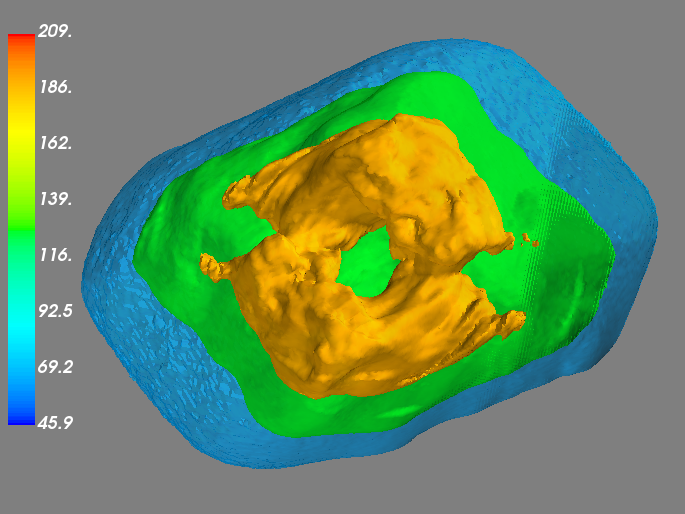
\includegraphics[height=8em]{figures/5a1a_aligned}
        \caption{Reconstructed $\widehat{\x}$ from $\{ \p_i, \widehat{q_i} \}$.}%
        \label{fig:5a1a-noise0-reconstruction-recovered}
    \end{subfigure}
    \hfill
    \begin{subfigure}[b]{0.26\linewidth}
        \centering
        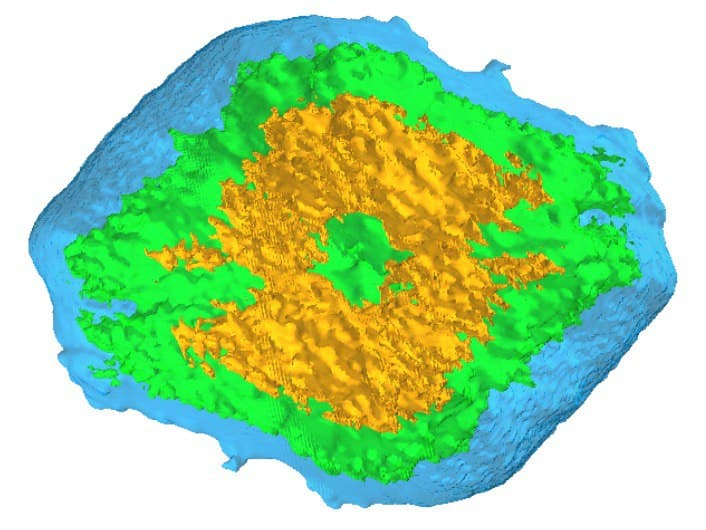
\includegraphics[height=8em]{figures/5a1a_ground_truth}
        \caption{Reconstructed $\widehat{\x}$ from $\{ \p_i, q_i \}$.}%
        \label{fig:5a1a-noise0-reconstruction-true}
    \end{subfigure}
    \caption{%
        Orientation recovery and density reconstruction from estimated distances.
        The first column~(a,d,g) shows orientation recovery:
        The blue curve shows the evolution of the recovery loss until convergence, with the minimum $L_\text{OR}$ \eqnref{orientation-recovery} highlighted.
        The red histogram shows the errors in the recovered orientations $\{d_q(q_i, \mathbf{T}\widehat{q_i})\}$, with the mean $E_\text{OR}$ \eqnref{orientation-recovery-error} highlighted.
    The second and third columns show density maps $\widehat{\x}$ reconstructed from projections $\{ \p_i \}$, and recovered orientations $\{ \widehat{q_i} \}$~(b,e,h) or true orientations $\{ q_i \}$~(c,f,i).
        % Explain columns then rows.
        The first row~(a,b,c) shows the process for noiseless projections $\p_i = \mathbf{P}_{\bth_i} \x$, where $\x$ comes from \texttt{5j0n}.
        \mdeff{Why is $L_\text{OR} = 0.05$ while it is $0.01$ in \figref{results:distance-estimation:noise}?}
        The second row~(d,e,f) shows the process for noisy projections $\p_i = \mathbf{P}_{\bth_i} \x + \mathbf{n}$, where $\mathbf{n} \sim \mathcal{N}(0, \sigma^2\mathbf{I}), \sigma^2=16$, and $\x$ comes from \texttt{5j0n}.
        \mdeff{$E_\text{OR}=0.4184$ is the same as for $\sigma^2=15$ (\figref{results:distance-estimation:noise}). Coincidence or error?}
        The third row~(g,h,i) shows the process for noiseless projections $\p_i = \mathbf{P}_{\bth_i} \x$, where $\x$ comes from \texttt{5a1a}.
        \mdeff{It would be clearer here to have $P_{q_i}$ instead of $P_{\bth_i}$ but we didn't introduce this notation. Should we?}
    }
\end{figure}

\figref{5j0n-noise0-orientation-recovery} shows the recovery of orientations from distances estimated from clean projections of \texttt{5j0n}.
A mean error of $E_\text{OR} \approx 0.16$ radians ($\approx 9\degree$) in the recovered orientations led to a \todo{pretty good?} reconstruction (\figref{5j0n-noise0-reconstruction-recovered}) compared to that with true orientations (\figref{5j0n-noise0-reconstruction-true}).
\mdeff{I'm not sure how to qualify the reconstructed density maps.}

As expected from the experiments in \secref{results:distance-estimation:sensitivity}, adding white noise with variance $\sigma^2=16$ to the projections worsen the recovered orientations (\figref{5j0n-noise16-orientation-recovery}) to a mean error of $E_\text{OR} \approx 0.42$ radians ($\approx 24\degree$).
That leads to a \todo{worse/lower resolution/blurrier} reconstruction (\figref{5j0n-noise16-reconstruction-recovered}).
Note that reconstructing from true orientations worsen too  (\figref{5j0n-noise16-reconstruction-true}) as the projections themselves are degraded.

Finally, \figref{5a1a-noise0-orientation-recovery} shows the recovery of orientations from clean projections of \texttt{5a1a}.
A mean error of $E_\text{OR} \approx 0.19$ radians ($\approx 11\degree$) in the recovered orientations led to a \todo{blurrier} reconstruction (\figref{5j0n-noise0-reconstruction-recovered}) compared to that with true orientations (\figref{5j0n-noise0-reconstruction-true}).
Orientation recovery is slightly more difficult for this protein \todo{as distance estimation is more difficult because} \mdeff{Symmetries? Something else? What makes \texttt{5a1a} harder than \texttt{5j0n}?}.

%We observe that the recovery of more accurate orientations lead to the reconstruction of more accurate density maps.
%Hence, the estimation of more accurate distances lead to more accurate reconstructions.
We observe that the estimation of more accurate distances not only lead to the recovery of more accurate orientations, but also to the reconstruction of more accurate density maps.
%Reconstruction is most affected by the presence of noise, due to the degraded estimation of distances.
We are hence confident that reconstruction would substantially improve if a more powerful SiameseNN would be trained on more data for distance estimation (and a \todo{more serious/advanced/less naive?} method used for reconstruction).
%\mdeff{Story: pipeline works but better distance estimation is needed for SOTA reconstruction.
%Method is however promising because learned distance is robust to perturbations and recovery works if distance works.}
